\documentclass[border=15pt, multi, tikz]{article}
\usepackage[backend=bibtex,style=authoryear,natbib=true]{biblatex} % Use the bibtex backend with the authoryear citation style (which resembles APA)

\addbibresource{example.bib} % The filename of the bibliography

\usepackage[autostyle=true]{csquotes} % Required to generate language-dependent quotes in the bibliography
\usepackage{import}
\usepackage{tikz}
\usepackage{tikz-network}
\usetikzlibrary{calc,patterns,angles,quotes}
\usepackage{breqn}
\usepackage{bm}
\usepackage{float}
\usepackage{graphicx}
\usepackage{subcaption}
\usepackage{multirow}
\usepackage{graphicx}
\usepackage{rotating}
\usetikzlibrary{fit}
\usetikzlibrary {arrows.meta,graphs,shapes.misc}
\usetikzlibrary {positioning}
\subimport{./layers/}{init}
\newcommand{\bn}{\textbf{n}}
\newcommand{\tabhead}[1]{\textbf{#1}}

\def\ConvColor{rgb:yellow,5;red,2.5;white,5}
\def\ConvReluColor{rgb:yellow,5;red,5;white,5}
\def\PoolColor{rgb:red,1;black,0.3}
\def\DcnvColor{rgb:blue,5;green,2.5;white,5}
\def\SoftmaxColor{rgb:magenta,5;black,7}
\def\SumColor{rgb:blue,5;green,15}
\def\poolsep{1}


\begin{document}
	
The approaches are trained on dataset "synthetic-50-5" as mentioned in Chapter \ref{ch:04} with 3000 scenes. The input matrix has $ 128\times 128 $ height and width. Each vertex map has dimension $ 128\times 128\times3 $, light map has $ 128\times 128 \times 3 $, image has dimension $ 128\times 128 \times 1 $.  The training pipeline use batch size $ 8 $,  Adam optimizer (\cite{adam}), learning rate of  $ 1\times10^{-3} $, learning schedule [8,1000], learning decay factor 0.5. 
The model is trained with PyTorch 1.10.0a0, CUDA 11.4.1, GPU with single NVIDIA GEFORCE RTX 3090. 


\section{GCNN model evaluation}
The GCNN model is the base model of the whole thesis. In this section, we first evaluate the inpainting performance of the model based on light map input. Then we use the same model for normal inference task.


\subsection{Light Inpainting}
The light inpainting task in this section in order to evaluate the noise inpainting performance of GCNN model. It takes semi-dense light map as input to predict the fully dense light map, as shown in Figure \ref{fig:light-net-archi}. 
The network is trained on 3000 light maps in the "synthetic-50-5" dataset with initial learning rate 0.001, learning schedule 8,1000 with decay factor 0.5, the batch size is 8, the feature map channel is 128 in all of the gated convolution layers. All the models are tested on a laptop with a single NVIDIA GeForce 940MX, 2GB memory.

%% light eval model structure
\begin{figure}[th]
	\centering
	%% https://tex.stackexchange.com/questions/12020/what-is-the-easiest-way-to-draw-a-3d-cube-with-tikz
	\begin{tikzpicture}
		%% -------------------------------------- parameters ------------------------------------------------
		\pgfmathsetmacro{\vdist}{0.4}
		
		\pgfmathsetmacro{\boxsizea}{2}	%% width 512
		\pgfmathsetmacro{\boxwidtha}{2}	%% width 3
		
		%% https://www.tug.org/pracjourn/2007-4/walden/color.pdf
		\definecolor{netcolor}{rgb}{0.5,0.7,0.7}
		
		%% 	d_in							3x512x512
		%%	dconv1: 	d_in-->x1 			32x512x512
		\pgfmathsetmacro{\disttimes}{1}	%% width 32
		\pgfmathsetmacro{\yshift}{1}	%% width 32
		\pgfmathsetmacro{\boxsize}{\boxsizea}	%% size 512
		\pgfmathsetmacro{\boxwidth}{\boxwidtha}	%% width 32
		\pgfmathsetmacro{\yschift}{-1}
		
		
		\node[inner sep=0pt] (input) at (\vdist*\disttimes-6,\yschift-0.8)
		{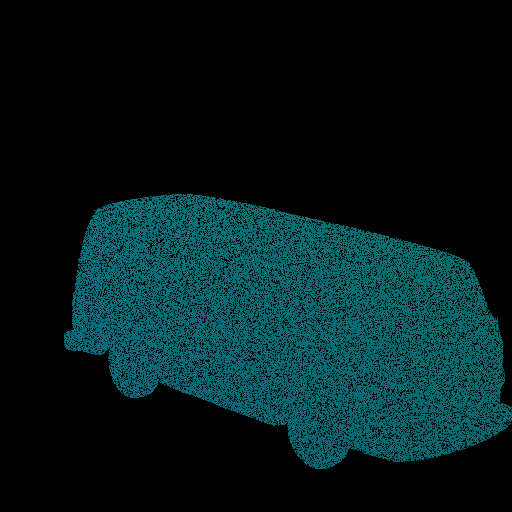
\includegraphics[width=.2\textwidth]{./Figures/gcnn-synthetic/intrinsic_image_light_input.png}};
		\node[text width=3.5cm] at (\vdist*\disttimes-6,\yschift-2.4) {Semi-dense Light Map};
		
		\node[inner sep=0pt] (output) at (\vdist*\disttimes+3,\yschift-0.8)
		{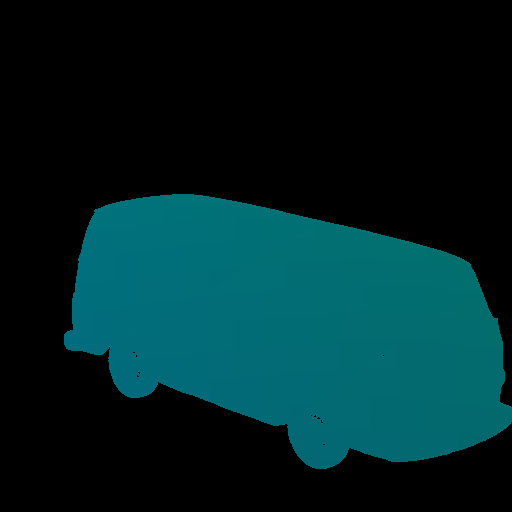
\includegraphics[width=.2\textwidth]{./Figures/gcnn-synthetic/intrinsic_image_light.png}};
		\node[text width=3.5cm] at (\vdist*\disttimes+3,\yschift-2.4) {fully-dense Light Map};
		
		\draw [-stealth] (\vdist*\disttimes-4.5,\yschift-1) -- (\vdist*\disttimes-3.5,\yschift-1);
		\draw [-stealth] (\vdist*\disttimes,\yschift-1) -- (\vdist*\disttimes+1,\yschift-1);
		
		
		\pgfmathsetmacro{\disttimes}{-2}	%% width 32		
		\pgfmathsetmacro{\yschift}{-1}
		\draw[black, fill=netcolor] (\vdist*\disttimes,\yschift,0) -- ++(-\boxwidth,0,0) -- ++(0,-\boxsize,0) -- ++(\boxwidth,0,0) -- cycle;
		\draw[black, fill=netcolor] (\vdist*\disttimes,\yschift,0) -- ++(0,0,-\boxsize) -- ++(0,-\boxsize,0) -- ++(0,0,\boxsize) -- cycle;
		\draw[black, fill=netcolor] (\vdist*\disttimes,\yschift,0) -- ++(-\boxwidth,0,0) -- ++(0,0,-\boxsize) -- ++(\boxwidth,0,0) -- cycle;
		
		\node[text width=3.5cm] at (\vdist*\disttimes+0.3,\yschift-1) {GCNN};
	\end{tikzpicture}
	\caption{Light map inpainting based on GCNN architecture.}
	\label{fig:light-net-archi}
\end{figure}

The result is shown in Table \ref{tab:light-inpainting}. Besides the GCNN model, we use two extra model as the comparisons. The first one is GCNN-NOC, where NOC means "no skip connection", the second one is CNN, which has the same architecture as the GCNN but only use standard convolution layers in the network.
The GCNN architecture achieves the average angle error lower than 1 degree. As a comparison, U-CNN model has 4 degrees error, which shows the relative weakness of noise filter competence. Besides, the skip connection also booster the performance, since the no skip connection version still has error greater than 1 degree. The both two models for the inpainting task reveals the superiority of GCNN architecture. Figure \ref{fig:light-scatter} and \ref{fig:light-eval} gives a quantitative and qualitative evaluation.

%% light eval table
\begin{table}[H]
	
	\centering
	\begin{tabular}{l l l l l l }
		\tabhead{Model} & \tabhead{Angle} & \tabhead{Time /ms} & \tabhead{bz} & \tabhead{lr-schedule} & \tabhead{lr-df}\\
		U-GCNN  & 0.59  & 14.45 & 8 & 8,1000 & 0.5\\ 
		\hline
		U-GCNN-NOC & 1.31 & 16.14 & 8 & 8,1000 & 0.5\\
		\hline
		U-CNN & 4.10 & 10.52 & 8 & 8,1000 & 0.5\\
	\end{tabular}
	\caption{The performance of the GCNN model for light map inpainting. The angle error is the average angle error of all valid pixels in the test case. bz stands for batch size, lr-schedule stands for learning rate schedule, lr-df stands for learning rate decay factor.}	
	\label{tab:light-inpainting}
\end{table}


%% light eval visualization
\begin{figure}[H]
	\centering
	\begin{subfigure}[b]{0.24\linewidth}
		\includegraphics[width=\linewidth]{./Figures/gcnn-light/fancy_eval_1_img.png}
		\caption{gray-scale image}
	\end{subfigure}
	\begin{subfigure}[b]{0.24\linewidth}
			\includegraphics[width=\linewidth]{./Figures/gcnn-light/fancy_eval_1_light_input.png}
		\caption{Vertex(Input)}
	\end{subfigure}
	\begin{subfigure}[b]{0.24\linewidth}
		
\includegraphics[width=\linewidth]{./Figures/gcnn-light/fancy_eval_1_light_gt.png}
		\caption{ground-truth}
	\end{subfigure}

	\begin{subfigure}[b]{0.24\linewidth}
	
\includegraphics[width=\linewidth]{./Figures/gcnn-light/fancy_eval_1_light_light.png}
		\caption{GCNN}
	\end{subfigure}
	\begin{subfigure}[b]{0.24\linewidth}
	
\includegraphics[width=\linewidth]{./Figures/gcnn-light/fancy_eval_1_light_light-cnn.png}
	\caption{U-CNN}
\end{subfigure}
	\begin{subfigure}[b]{0.24\linewidth}
	
\includegraphics[width=\linewidth]{./Figures/gcnn-light/fancy_eval_1_light_light-noc.png}
	\caption{U-GCNN-NOC}
\end{subfigure}

	\begin{subfigure}[b]{0.24\linewidth}
	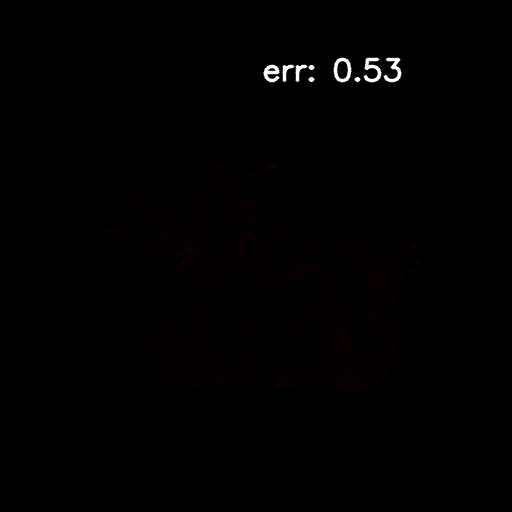
\includegraphics[width=\linewidth]{./Figures/gcnn-light/fancy_eval_1_light_error_light.png}
	\caption{U-GCNN Error}
	\end{subfigure}
	\begin{subfigure}[b]{0.24\linewidth}
	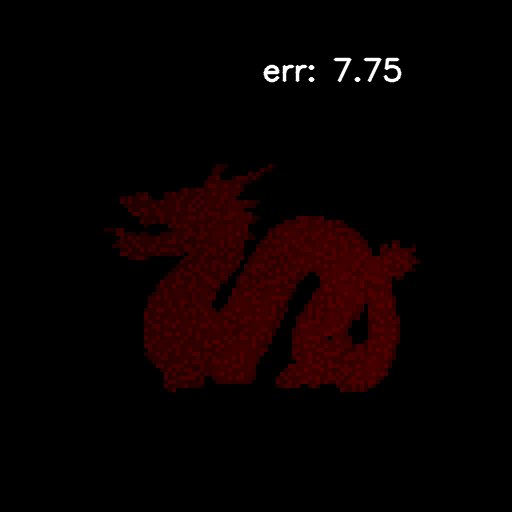
\includegraphics[width=\linewidth]{./Figures/gcnn-light/fancy_eval_1_light_error_light-cnn.png}
	\caption{U-CNN Error}
	\end{subfigure}
	\begin{subfigure}[b]{0.24\linewidth}
	
\includegraphics[width=\linewidth]{./Figures/gcnn-light/fancy_eval_1_light_error_light-noc.png}
	\caption{U-NOC Error}
	\end{subfigure}

	\begin{tikzpicture}
	\node[text width=0.1\textwidth] at (10,-1) {90};
	\node[inner sep=0pt] (input) at (8,-1)
	{
\includegraphics[width=.2\textwidth]{./Figures/colorscale_hot-vertical.jpg}};
	\node[text width=0.3\textwidth] at (7,-1) {Error: 0};
	\end{tikzpicture}

	\caption{GCNN Normal Inference for light map inpainting based on dragon object. The degree error map is shown in last row. The average error is shown in the upper right corner in the error map.}
	\label{fig:light-eval}
\end{figure}

%% light eval scatter
\begin{figure}[H]
	\centering
	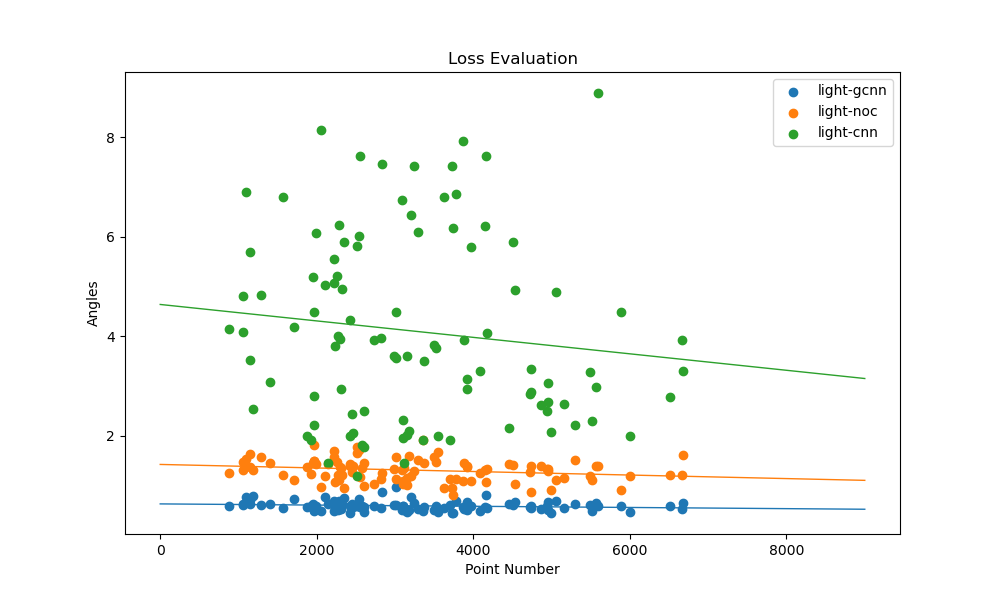
\includegraphics[width=0.9\linewidth]{./Figures/gcnn-light/scatter-light.png}
	\caption{GCNN for light map inpainting on 100 scenes. The evaluated models are corresponding to the table \ref{tab:light-inpainting}, the line in the figure is the corresponding regression line of each model.}
	\label{fig:light-scatter}
\end{figure}




%% nnnn exp
\subsection{Surface Normal Inference}

We evaluate geometry based approach for surface normal estimation using a pure GCNN architecture.  The input of the model is 3D vertex map whereas the output is directly the corresponding tangent surface normal map in range $ [-1,1] $. The training parameters are as same as light inpainting task mentioned above.

A qualitative evaluation on object "dragon" is shown in Figure \ref{fig:gcnn-eval-synthetic} and Figure \ref{fig:gcnn-eval-synthetic-zoom-in}, theb SVD approach is considered as a base line. The GCNN based approach has apparently better performance than SVD based approach, which completely get rid of the trace of the noise in the input vertex map. Figure \ref{fig:gcnn-eval-synthetic-zoom-in} zooms in the right leg area of the Washington statue object to give a closer comparison with the ground-truth.
As shown in the figure, the GCNN method successfully predict the surface connection area between the lower hem of the gown and the stone chair, whereas the no skip version is blurry in the same area. The two surface is still distinguishable but the sharp details has been lost.  The CNN version has the skip connection thus gives a better detail than NOC version. However, if we compare the error map of U-GCNN and U-CNN in figure \ref{fig:gcnn-eval-synthetic}, the basement of the stone chair that Washington sit is actually a smooth flat stage, the U-GCNN shows an accurate predict, but the same area in U-CNN has an average higher error. The whole basement surface has a overall higher error. It holds also for the other smooth areas like the side of the stone chair, the gown and the upper body of the statue. It is because the noise of the input still disturb the CNN model and take the input noise into account for normal estimation which deviate to the correct surface normal. When we look back to the U-GCNN based method, we can found that the surface normal has better performance in the smooth area compare to the CNN approach and a sharp detail compare to the no skip connection version.


%% gcnn-eval
\begin{figure}[H]
	\centering
	\begin{subfigure}[b]{0.18\linewidth}
		\includegraphics[width=\linewidth]{./Figures/gcnn-synthetic/fancy_eval_5_groundtruth.png}
	\end{subfigure}
	\begin{subfigure}[b]{0.18\linewidth}
		\includegraphics[width=\linewidth]{./Figures/gcnn-synthetic/fancy_eval_5_normal_GCNN-GCNN.png}
	\end{subfigure}
	\begin{subfigure}[b]{0.18\linewidth}
		\includegraphics[width=\linewidth]{./Figures/gcnn-synthetic/fancy_eval_5_normal_GCNN-CNN.png}
	\end{subfigure}
	\begin{subfigure}[b]{0.18\linewidth}
		\includegraphics[width=\linewidth]{./Figures/gcnn-synthetic/fancy_eval_5_normal_GCNN-NOC.png}
	\end{subfigure}
	\begin{subfigure}[b]{0.18\linewidth}
		\includegraphics[width=\linewidth]{./Figures/gcnn-synthetic/fancy_eval_5_normal_SVD.png}
	\end{subfigure}
	
	\begin{subfigure}[b]{0.18\linewidth}
		\includegraphics[width=\linewidth]{./Figures/gcnn-synthetic/fancy_eval_5_img.png}
		\caption{GT}
	\end{subfigure}
	\begin{subfigure}[b]{0.18\linewidth}
		\includegraphics[width=\linewidth]{./Figures/gcnn-synthetic/fancy_eval_5_error_GCNN-GCNN.png}
		\caption{U-GCNN}
	\end{subfigure}
	\begin{subfigure}[b]{0.18\linewidth}
		\includegraphics[width=\linewidth]{./Figures/gcnn-synthetic/fancy_eval_5_error_GCNN-CNN.png}
		\caption{U-CNN}
	\end{subfigure}
	\begin{subfigure}[b]{0.18\linewidth}
		\includegraphics[width=\linewidth]{./Figures/gcnn-synthetic/fancy_eval_5_error_GCNN-NOC.png}
		\caption{U-NOC}
	\end{subfigure}
	\begin{subfigure}[b]{0.18\linewidth}
	\includegraphics[width=\linewidth]{./Figures/gcnn-synthetic/fancy_eval_5_error_SVD.png}
	\caption{SVD}
	\end{subfigure}
	
	\begin{tikzpicture}
		\node[text width=0.1\textwidth] at (10,-1) {90};
		\node[inner sep=0pt] (input) at (8,-1)
		{
\includegraphics[width=.2\textwidth]{./Figures/colorscale_blue.png}};
		\node[text width=0.3\textwidth] at (7,-1) {Error: 0};
	\end{tikzpicture}
	
	\caption{Surface Normal Inference based GCNN model on "Washington´´ object. The first row shows the estimated surface normal. The second row is the degree error map.}
	\label{fig:gcnn-eval}
\end{figure}

%% fig:gcnn-eval-synthetic-zoom-in
\begin{figure}[H]
	\centering
	\begin{subfigure}[b]{0.18\linewidth}
		\includegraphics[width=\linewidth]{./Figures/gcnn-synthetic/eval_5_normal_GT.png}
	\end{subfigure}
	\begin{subfigure}[b]{0.18\linewidth}
		\includegraphics[width=\linewidth]{./Figures/gcnn-synthetic/eval_5_normal_GCNN-GCNN.png}
	\end{subfigure}
	\begin{subfigure}[b]{0.18\linewidth}
		\includegraphics[width=\linewidth]{./Figures/gcnn-synthetic/eval_5_normal_GCNN-NOC.png}
	\end{subfigure}
	\begin{subfigure}[b]{0.18\linewidth}
		\includegraphics[width=\linewidth]{./Figures/gcnn-synthetic/eval_5_normal_GCNN-CNN.png}
	\end{subfigure}
	\begin{subfigure}[b]{0.18\linewidth}
	\includegraphics[width=\linewidth]{./Figures/gcnn-synthetic/eval_5_normal_SVD.png}
	\end{subfigure}

	\begin{subfigure}[b]{0.18\linewidth}
		\includegraphics[width=\linewidth]{./Figures/gcnn-synthetic/eval_5_img.png}
		\caption{GT}
	\end{subfigure}
	\begin{subfigure}[b]{0.18\linewidth}
		\includegraphics[width=\linewidth]{./Figures/gcnn-synthetic/eval_5_error_GCNN-GCNN.png}
		\caption{GCNN}
	\end{subfigure}
	\begin{subfigure}[b]{0.18\linewidth}
		\includegraphics[width=\linewidth]{./Figures/gcnn-synthetic/eval_5_error_GCNN-NOC.png}
		\caption{NOC}
	\end{subfigure}
	\begin{subfigure}[b]{0.18\linewidth}
		\includegraphics[width=\linewidth]{./Figures/gcnn-synthetic/eval_5_error_GCNN-CNN.png}
		\caption{CNN}
	\end{subfigure}
	\begin{subfigure}[b]{0.18\linewidth}
	\includegraphics[width=\linewidth]{./Figures/gcnn-synthetic/eval_5_error_SVD.png}
	\caption{SVD}
	\end{subfigure}

	\caption{Zoom in of the center region of Washington object. The first row is surface normal, the second row is the corresponding errors.}
	\label{fig:gcnn-eval-synthetic-zoom-in}
\end{figure}




The evaluation visualization on real dataset is shown in Figure \ref{fig:gcnn-eval-real}
%% fig:gcnn-eval-real
\begin{figure}[th]
	\centering
	\begin{subfigure}[b]{0.24\linewidth}
		
\includegraphics[width=\linewidth]{./Figures/gcnn-real/fancy_eval_1_point_cloud_noise.png}
		\caption{point cloud}
	\end{subfigure}
	\begin{subfigure}[b]{0.24\linewidth}
		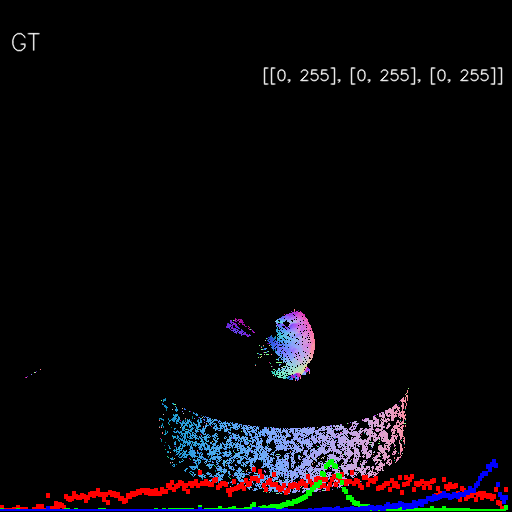
\includegraphics[width=\linewidth]{./Figures/gcnn-real/fancy_eval_1_groundtruth.png}
		\caption{ground-truth}
	\end{subfigure}
	\begin{subfigure}[b]{0.24\linewidth}
		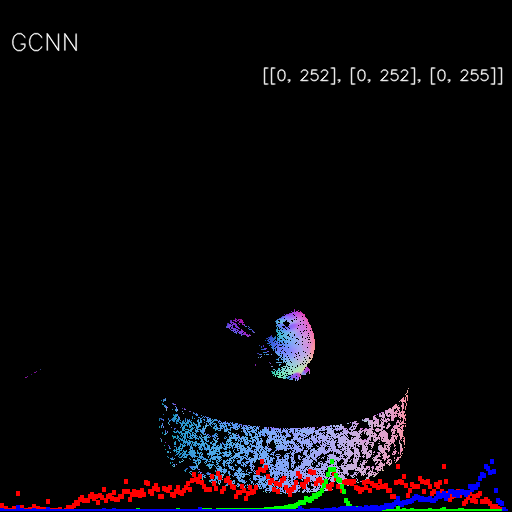
\includegraphics[width=\linewidth]{./Figures/gcnn-real/fancy_eval_1_normal_GCNN.png}
		\caption{GCNN}
	\end{subfigure}
	\begin{subfigure}[b]{0.24\linewidth}
		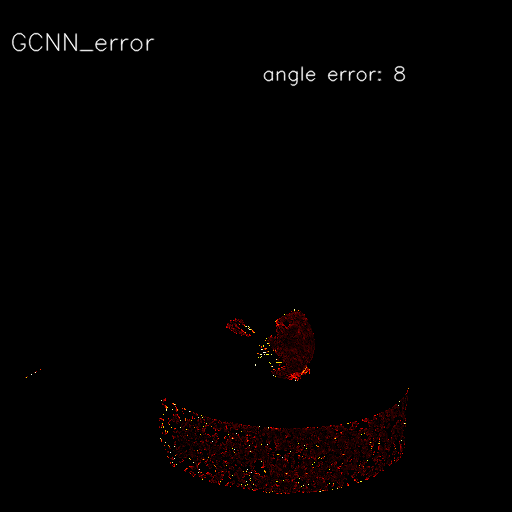
\includegraphics[width=\linewidth]{./Figures/gcnn-real/fancy_eval_1_error_GCNN.png}
		\caption{Angle Error}
	\end{subfigure}
	\caption{Evaluation on Real Dataset}
	\label{fig:gcnn-eval-real}
\end{figure}


We evaluate the U-GCNN model on 100 test images as a quantitative evaluation. The result is shown in Figure \ref{fig:scatter-gcnn}. The GCNN based method has average angle error around 10 degrees, whereas the no skip connection version has error above 12 degrees and the CNN version has error above 15 degrees.

%% scatter_gcnn
\begin{figure}[h!]
	\centering
	\includegraphics[width=.8\textwidth]{./Figures/gcnn-synthetic/gcnn-scatter.png}
	\caption{Evaluation of average angular loss on the whole test dataset with 100 scenes. The x-axis indicates the point number, the y-axis indicates the angles. The lines show in the picture are the regression line of each model.}
	\label{fig:scatter-gcnn}
\end{figure}


\newpage
\section{Surface Normal Inference based on Calibrated Illuminated RGBD images }

\subsection{Light Net Evaluation}

We evaluate the GCNN architecture based light net on the test dataset. The light net parameters are further used as the initial parameter of light branch of the Trignet.

A qualitative evaluation of light net is shown in Figure \ref{fig:eval-light}. The average angular error are lower than $ 0.3 $ degree on all of test cases. In this case, to distinguish the output and the ground truth is already not easily only use naked eyes. 


\begin{figure}[th]
	\centering
	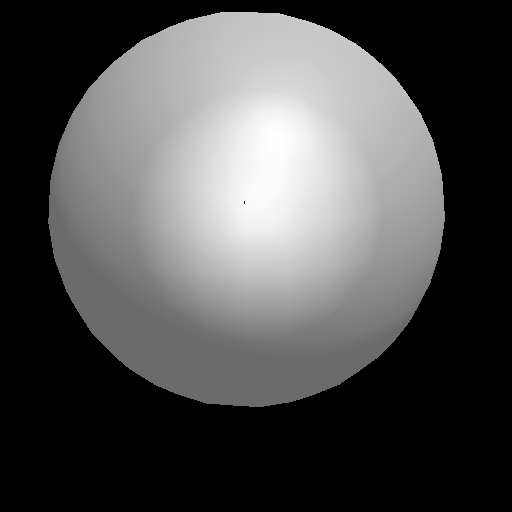
\includegraphics[width=0.18\linewidth]{./Figures/light-synthetic/fancy_eval_0_img.png}
	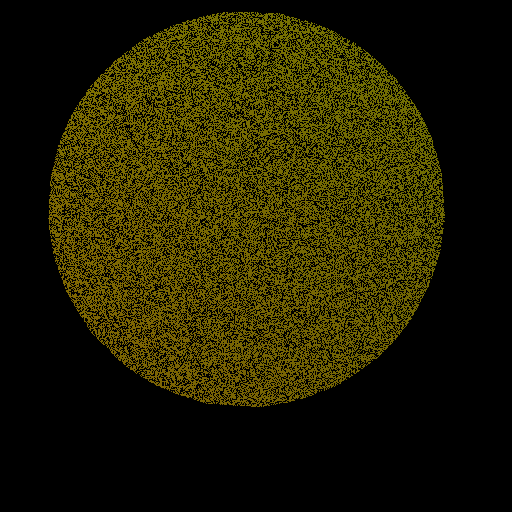
\includegraphics[width=0.18\linewidth]{./Figures/light-synthetic/fancy_eval_0_light_input.png}
	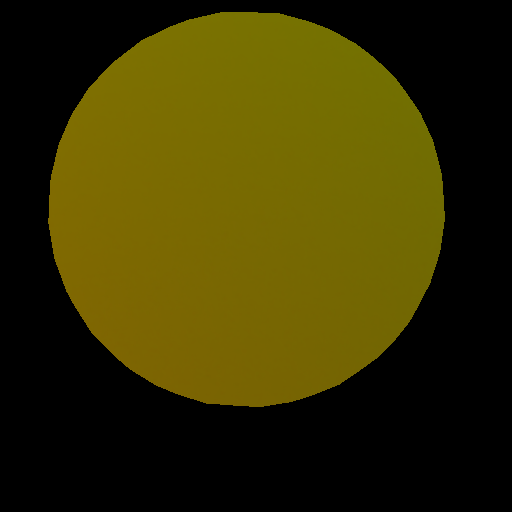
\includegraphics[width=0.18\linewidth]{./Figures/light-synthetic/fancy_eval_0_light_light.png}
	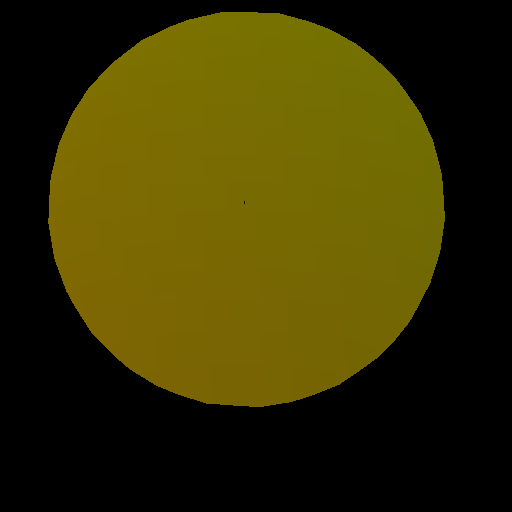
\includegraphics[width=0.18\linewidth]{./Figures/light-synthetic/fancy_eval_0_light_gt.png}
	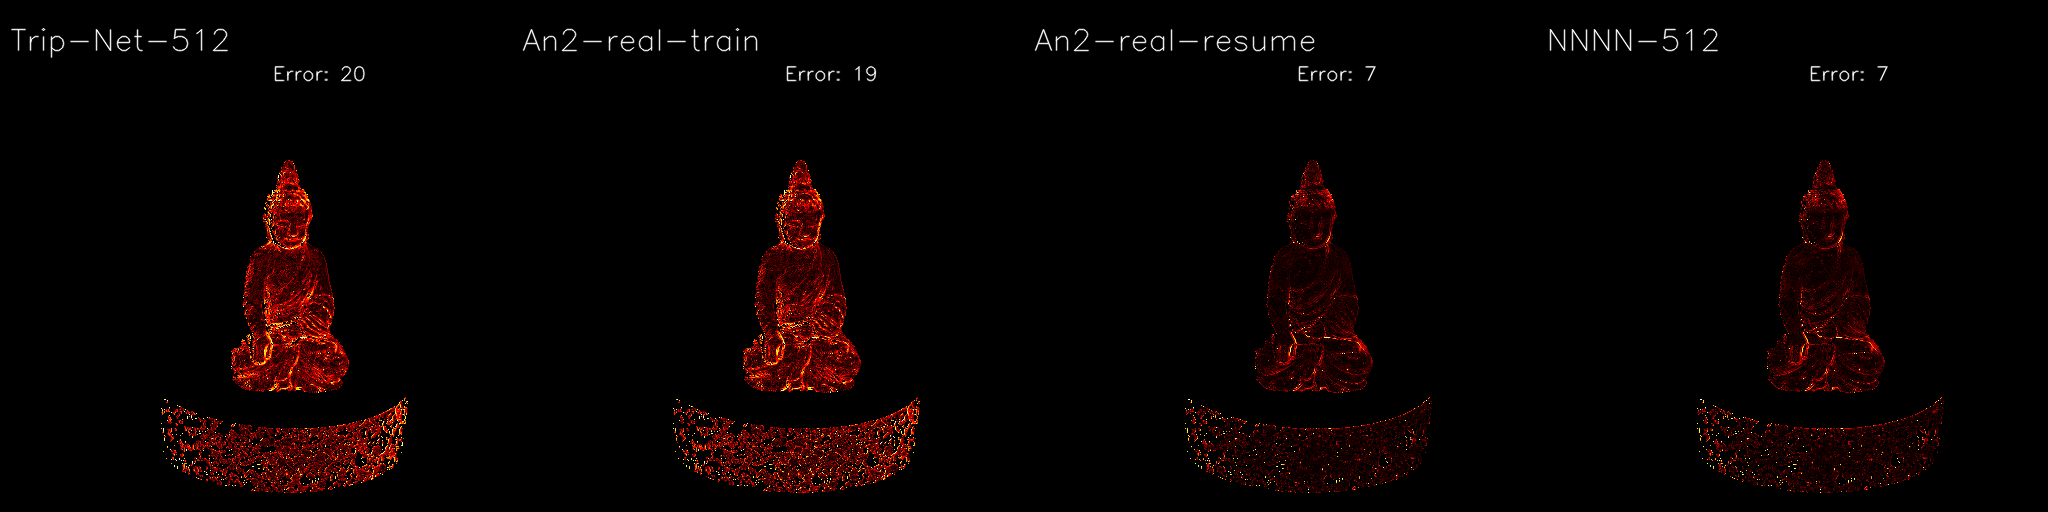
\includegraphics[width=0.18\linewidth]{./Figures/light-synthetic/fancy_eval_0_output_error.png}
	
	\includegraphics[width=0.18\linewidth]{./Figures/light-synthetic/fancy_eval_1_img.png}
	\includegraphics[width=0.18\linewidth]{./Figures/light-synthetic/fancy_eval_1_light_input.png}
	
\includegraphics[width=0.18\linewidth]{./Figures/light-synthetic/fancy_eval_1_light_light.png}
	
\includegraphics[width=0.18\linewidth]{./Figures/light-synthetic/fancy_eval_1_light_gt.png}
	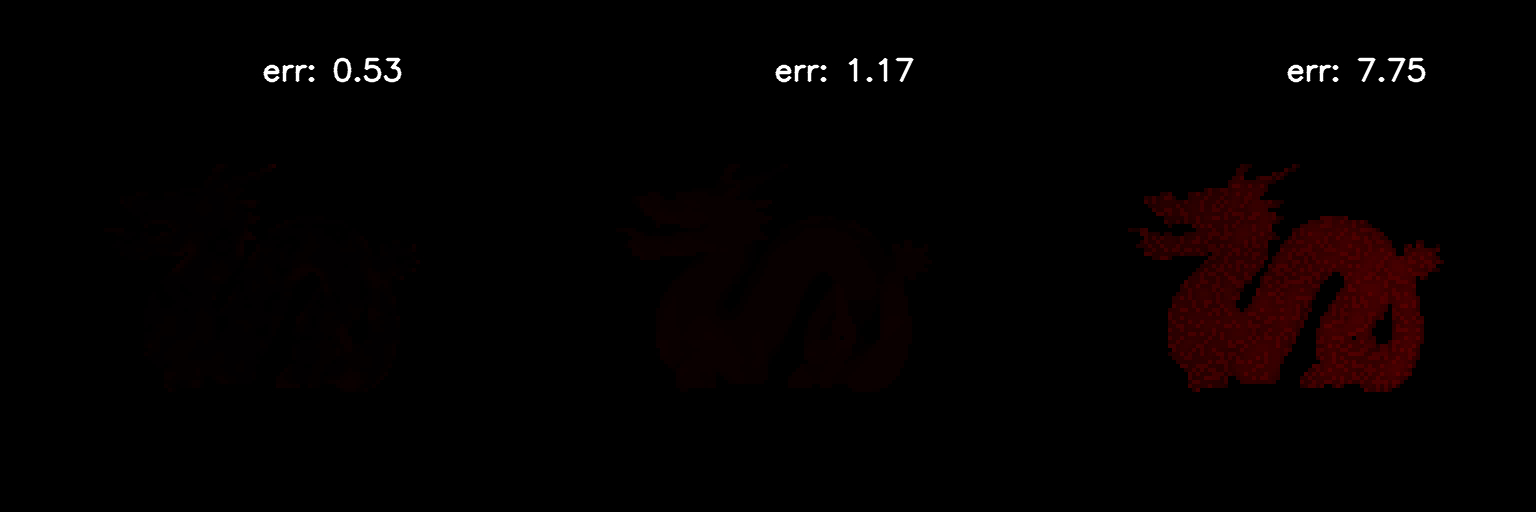
\includegraphics[width=0.18\linewidth]{./Figures/light-synthetic/fancy_eval_1_output_error.png}
	
	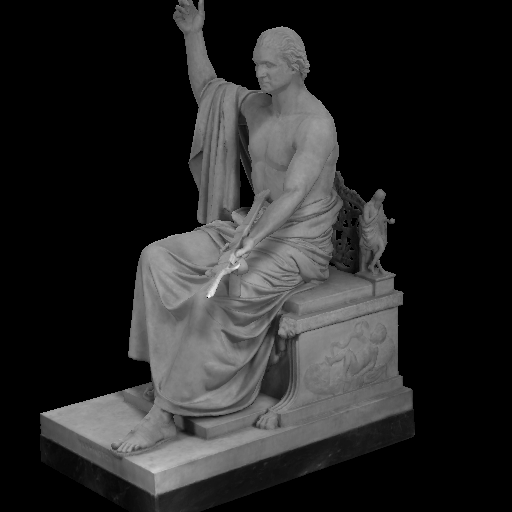
\includegraphics[width=0.18\linewidth]{./Figures/light-synthetic/fancy_eval_4_img.png}
	\includegraphics[width=0.18\linewidth]{./Figures/light-synthetic/fancy_eval_4_light_input.png}
	\includegraphics[width=0.18\linewidth]{./Figures/light-synthetic/fancy_eval_4_light_light.png}
	\includegraphics[width=0.18\linewidth]{./Figures/light-synthetic/fancy_eval_4_light_gt.png}
	\includegraphics[width=0.18\linewidth]{./Figures/light-synthetic/fancy_eval_4_output_error.png}
	
	\caption{Qualitative evaluation of light net on Sphere, bus and Washington statue. From left to right, grayscale image, semi-dense light map(input), full-dense light map(output), full-dense light map(ground-truth), error map.}
	\label{fig:eval-light}
\end{figure}

Figure \ref{fig:scatter-light} uses a scatter plot to show the average angular error on 100 different test cases. The average pixel-wise angular error is 0.17 degree as shown in Table \ref{tab:model-error}. An regression line has been added in the plot to analysis the tendency of the errors. The angular error slightly goes up when valid point number in the scene increase. It is make sense since the valid pixels are usually connected and concentrate in a single patch, the less of the area of the patch, which corresponding the number of the valid points, the less variation of the light direction among the pixels, thus better the evaluation.


\begin{figure}[th]
	\centering
	\includegraphics[width=0.5\linewidth]{./Figures/scatter-light-noised.png}
	\caption{The evaluation on 100 test cases of Light Net.}
	\label{fig:scatter-light}
\end{figure}



\subsection{Vertex-Image-Light Net (VIL Net) Evaluation}


The qualitative evaluation of VIL net uses the model trained based on masked L2 loss.

\subsubsection{title}

\begin{figure}[th]
	\centering
	\includegraphics[width=0.18\linewidth]{./Figures/light-synthetic/fancy_eval_0_img.png}
	\includegraphics[width=0.18\linewidth]{./Figures/light-synthetic/fancy_eval_0_light_input.png}
	\includegraphics[width=0.18\linewidth]{./Figures/light-synthetic/fancy_eval_0_light_light.png}
	\includegraphics[width=0.18\linewidth]{./Figures/light-synthetic/fancy_eval_0_light_gt.png}
	\includegraphics[width=0.18\linewidth]{./Figures/light-synthetic/fancy_eval_0_output_error.png}
	
	\includegraphics[width=0.18\linewidth]{./Figures/light-synthetic/fancy_eval_1_img.png}
	\includegraphics[width=0.18\linewidth]{./Figures/light-synthetic/fancy_eval_1_light_input.png}
	\includegraphics[width=0.18\linewidth]{./Figures/light-synthetic/fancy_eval_1_light_light.png}
	\includegraphics[width=0.18\linewidth]{./Figures/light-synthetic/fancy_eval_1_light_gt.png}
	\includegraphics[width=0.18\linewidth]{./Figures/light-synthetic/fancy_eval_1_output_error.png}
	
	\includegraphics[width=0.18\linewidth]{./Figures/light-synthetic/fancy_eval_4_img.png}
	\includegraphics[width=0.18\linewidth]{./Figures/light-synthetic/fancy_eval_4_light_input.png}
	\includegraphics[width=0.18\linewidth]{./Figures/light-synthetic/fancy_eval_4_light_light.png}
	\includegraphics[width=0.18\linewidth]{./Figures/light-synthetic/fancy_eval_4_light_gt.png}
	\includegraphics[width=0.18\linewidth]{./Figures/light-synthetic/fancy_eval_4_output_error.png}
	
	\caption{Qualitative evaluation of Trignet net on Sphere, bus and Washington statue. From left to right, semi 3D vertex map, full-dense normal map(output), full-dense normal map(ground-truth), error map.}
	\label{fig:eval-trignet}
\end{figure}

\begin{figure}[th]
	\centering
	\includegraphics[width=0.5\linewidth]{./Figures/scatter-light-noised.png}
	\caption{The evaluation on 100 test cases of Trignet.}
	\label{fig:scatter-trignet}
\end{figure}




\subsection{comparison}
From the Figure \ref{fig:normal-histo-diff} we can observe the normal difference between ground-truth and GCNN predicted normals in another dimension. It separates the interval $ \left[ -1,1 \right] $, which is exactly the range of normal vector, to 256 sections. Then it counts the number of points locates in each section for 3 axes.  The 3 axes are fitted quite well in most of interval but other than $ \left[ -0.25,0.25 \right] $ for x and y axes and  interval close to $ -1 $ for z axis. Therefore a further constraint can be considered to the loss function related to the normal difference shown in this figure.

It is faulty that almost no normal has -1 z-component in GCNN predicted normal map. The reason?
\begin{figure}[th]
	\centering
	\includegraphics[width=\linewidth]{./Figures/normal-histo-diff.png}
	\caption{The normal difference of between GCNN and ground-truth in x, y, z-axis respectively. The y axis indicates the number of points, x axis indicates the value of normal in x/y/z axis. (The chart is based on the "dragon" scene showing above)}
	\label{fig:normal-histo-diff}
\end{figure}


\begin{table}[th]
	
	\centering
	\begin{tabular}{l l l l l l l l }
		\tabhead{Model} & \tabhead{Angle} & \tabhead{Time /ms} & \tabhead{bz} & \tabhead{lr-schedule} & \tabhead{lr-df} & \tabhead{l/i. Nr.} & over-perform\\
		LightNet  & 0.17  & 4.72 & &  & & & \\ 
		\hline
		GCNN  & 10.57 & 5.25 & 8 & 200,1600 & 0.5 & 0 & - \\
		\hline
		an3 & 10.46 & 64.86 & 8 & 3,12,1000  & 0.5 & 1 & yes\\
		\hline
		an3 & 10.81 & 65.34 & 8 & 10,1000  & 0.5 & 1 & no(yes) \\
		\hline
		VIL-1 & 10.50 & 31.57 & 8 & 10,1000 & 0.5 & 1 & yes \\
		\hline
		VIL-1 & 10.82 & 32.61 & 8 & 3,12,1000 & 0.5 & 1 & no(yes) \\
		\hline
		VIL-3  & 10.79 & 54.76 & 8 & 100,1000 & 0.1 & 3 & no(yes) \\
		\hline
		VIL-10  & 11.10 & 132.32 & 8 & 100,1000 & 0.1 &10 & no(yes)\\
	\end{tabular}
	\caption{The error of models. The angle error is the average angle error of all valid pixels in the test case. The time unit is millisecond. bz is the batch size, lr-schedule is learning rate schedule. lr-df is learning rate decay factor, l/i. Nr is the number of light-image maps used for each scene}	
	\label{tab:model-error}
\end{table}


\begin{figure}[th]
	\centering
	\includegraphics[width=\linewidth]{./Figures/regression-comparison.png}
	\caption{The normal difference of between GCNN and ground-truth in x, y, z-axis respectively. The y axis indicates the number of points, x axis indicates the value of normal in x/y/z axis. (The chart is based on the "dragon" scene showing above)}
	\label{fig:normal-histo-diff}
\end{figure}




\end{document}
